\documentclass{csse4400}

% \teachermodetrue

\usepackage{languages}
\usepackage{float}

\title{Deploying with Terraform}
\author{Evan Hughes \& Brae Webb}

\date{\week{5}}
\begin{document}

\maketitle

\section{Before Class}
Ensure you have had practice using the AWS Academy Learner Lab.
It is preferable if you already have \link{Terraform installed}{https://learn.hashicorp.com/tutorials/terraform/install-cli}.
Please also have one of IntelliJ IDEA, PyCharm, or VSCode with the Terraform plugin installed.

\section{This Week}
This week we are going to deploy TaskOverflow our Todo Application to AWS using a hosted database and a single server website.

Specifically, this week you need to:
\begin{itemize}
    \item Authenticate Terraform to use the AWS Learner Lab.
    \item Configure an RDS database.
    \item [Path A] Configure a single server and deploy the container.
    \item [Path B] Configure an ECS cluster and deploy the container.
\end{itemize}

\section{Using Terraform in AWS Learner Labs}
Following the steps from the week four practical, start a Learner Lab in AWS Academy.
For this practical, you do not need to create any resources in the AWS Console.
The console can be used to verify that Terraform has correctly provisioned resources.

\begin{enumerate}
\item Once the Learner Lab has started, click on `AWS Details' to display information about the lab.

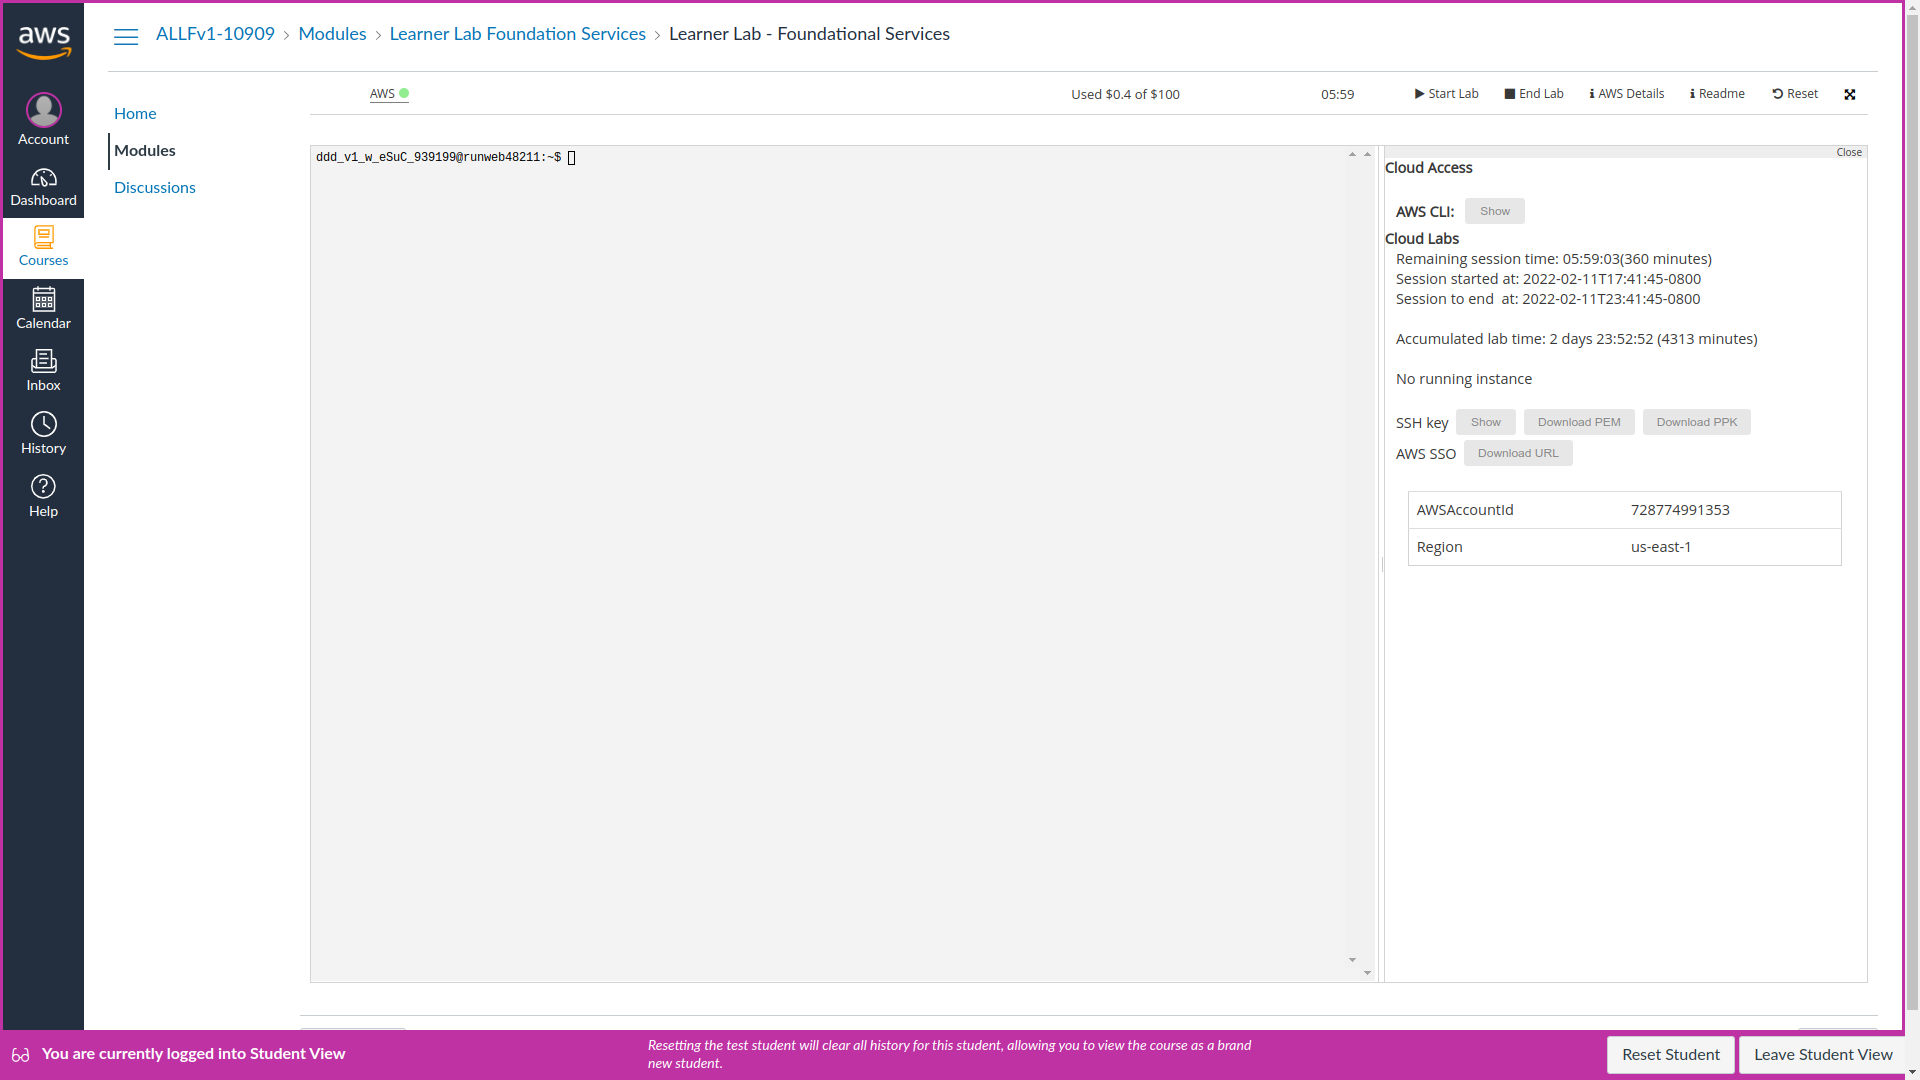
\includegraphics[width=0.7\textwidth]{images/aws-details}

\item Click on the first `Show' button next to `AWS CLI' which will display a text block starting with \texttt{[default]}.
\item Create a directory for this week's practical.
\item Within that directory create a \texttt{credentials} file and copy the contents of the text block into the file.
\textbf{Do \underline{not} share this file contents --- do \underline{not} commit it}.
\item Create a \texttt{main.tf} file in the same directory with the following contents:
\begin{code}[language=terraform]{main.tf}
terraform {
    required_providers {
        aws = {
            source  = "hashicorp/aws"
            version = "~> 4.0"
        }
    }
}

provider "aws" {
    region = "us-east-1"
    shared_credentials_files = ["./credentials"]
}
\end{code}

The \texttt{terraform} block specifies the required external dependencies, here we need to use the AWS provider.
The \texttt{provider} block configures the AWS provider, instructing it which region to use and how to authenticate (using the credentials file we created).

\item We need to initialise Terraform which will fetch the required dependencies. This is done with the \texttt{terraform init} command.
\bash{terraform init}

This command will create a \texttt{.terraform} directory which stores providers and a provider lock file, \texttt{.terraform.lock.hcl}.

\item To verify that we have setup Terraform correctly, use \texttt{terraform plan}.
\bash{terraform plan}

As we currently have no resources configured, it should find that no changes are required.
Note that this does not ensure our credentials are correctly configured as Terraform has no reason to try authenticating yet.

\end{enumerate}

\section{Deploying a Database in AWS}

\info{
This section manually deploys a Postgresql RDS instance, which is not the course's end goal but is a good way to get started with AWS. Later in this practical we will use Terraform to create the database, so this section is optional and is better to be observed rather than actioned.
}

\teacher{
  Instruct the class to observe you making the database and not to follow along.
}

\begin{figure}[ht]
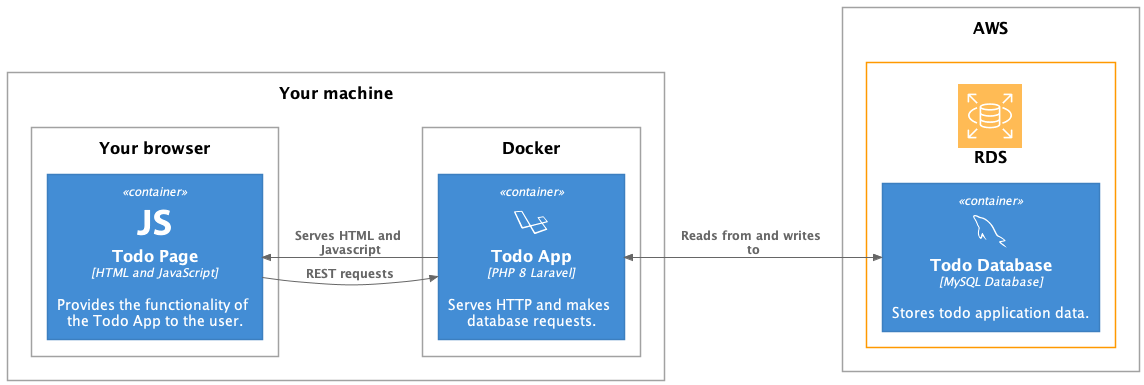
\includegraphics[width=\textwidth]{diagrams/remotedb}
\caption{Remote database deployment diagram}
\end{figure}

This is the last time we will heavily use the AWS user interface in the practicals. If you already feel confident in the AWS environment skip this section and move on to the next one.

\teacher{
  Give students time to start the labs, could take up to 10 minutes.
}

To get started let us jump into the lab environment and have a look at AWS RDS which is an AWS managed database service. To get to the RDS service either search it or browse Services -> Database -> RDS as shown below.

\begin{figure}[H]
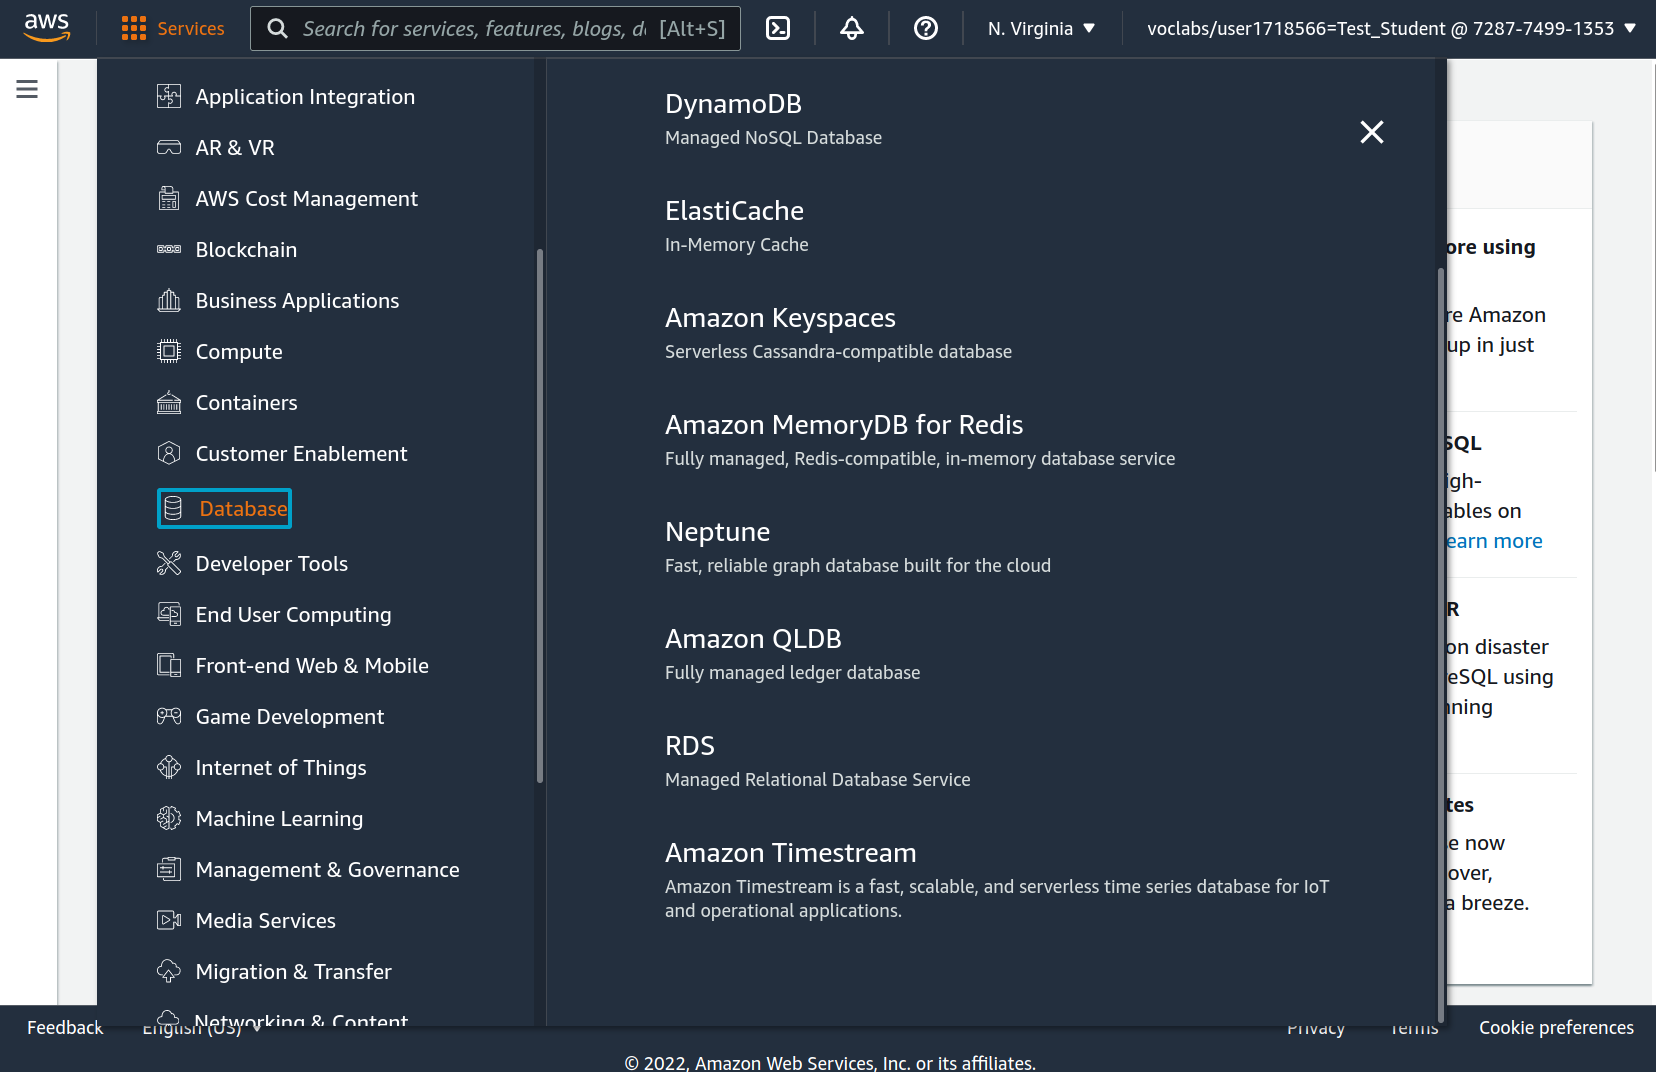
\includegraphics[width=\textwidth]{images/aws_1}
\end{figure}

Now we are in the management page for all our database instances,
for today we just want to get a small instance running to explore the service.
Head to ``DB Instances (0/40)''.

\begin{figure}[H]
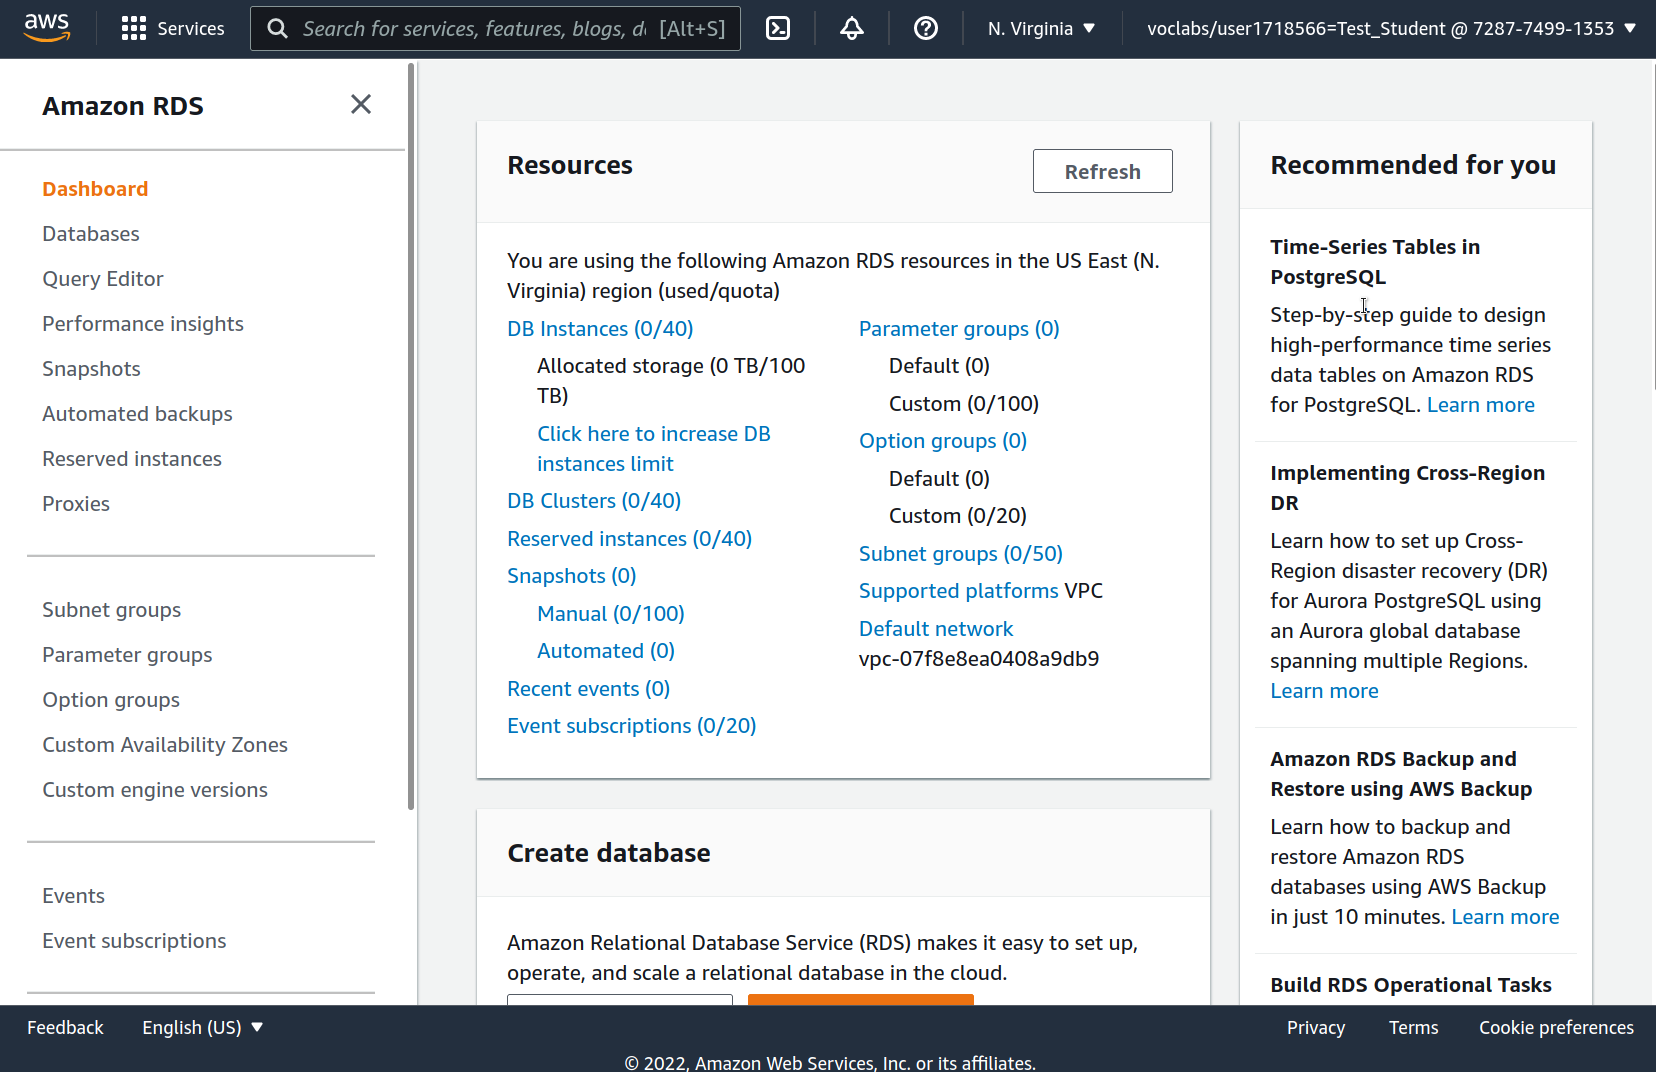
\includegraphics[width=\textwidth]{images/aws_2}
\end{figure}

This page should appear familiar as it is very similar to the AWS EC2 instance page.
Let us create a new database by hitting the ``Create Database'' button.

\begin{figure}[H]
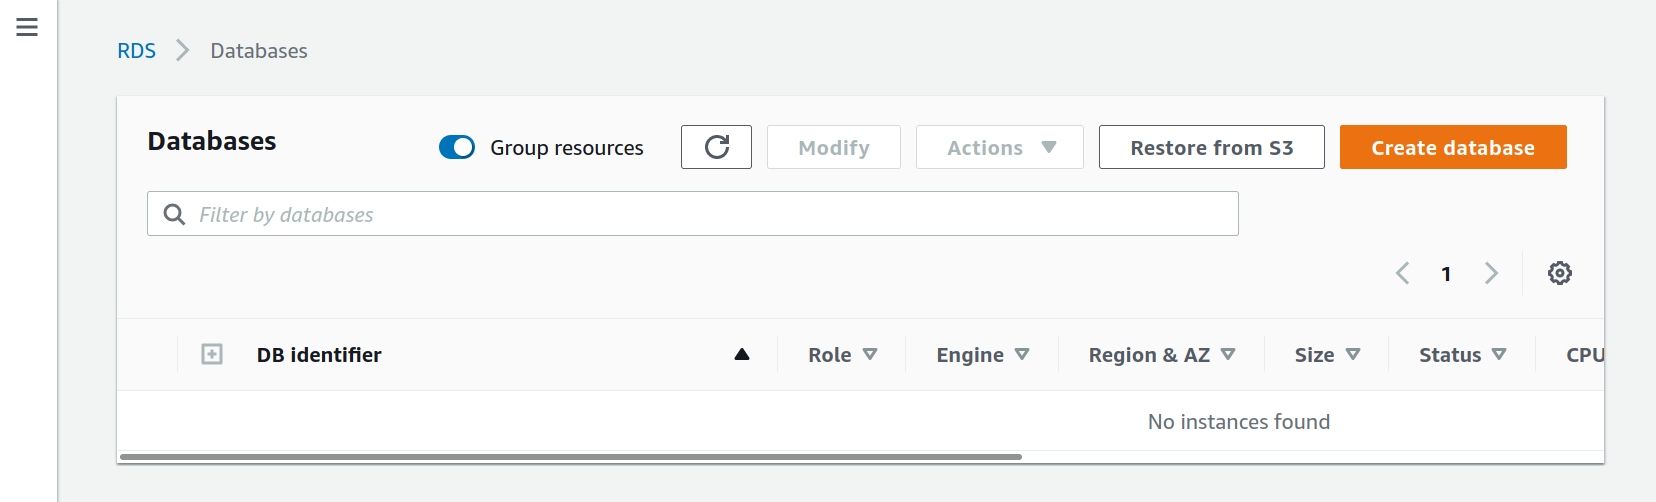
\includegraphics[width=\textwidth]{images/aws_3}
\end{figure}

\warning{
  In the next section we cannot use the Easy Create method as it tries to create a IAM account which is not allowed in the labs.
  Going forward we would typically do this using Terraform so we can easily avoid these restrictions.
}

\teacher{
  Feel free to talk about the other offerings here, but make sure to flame Oracle and Microsoft SQL Server.
  A good thing to point out is the Amazon Aurora which is the serverless version of RDS.
}

We will be creating a standard database so select standard and Postgresql.
We will use version 14, which is a fairly recent release.

\begin{figure}[H]
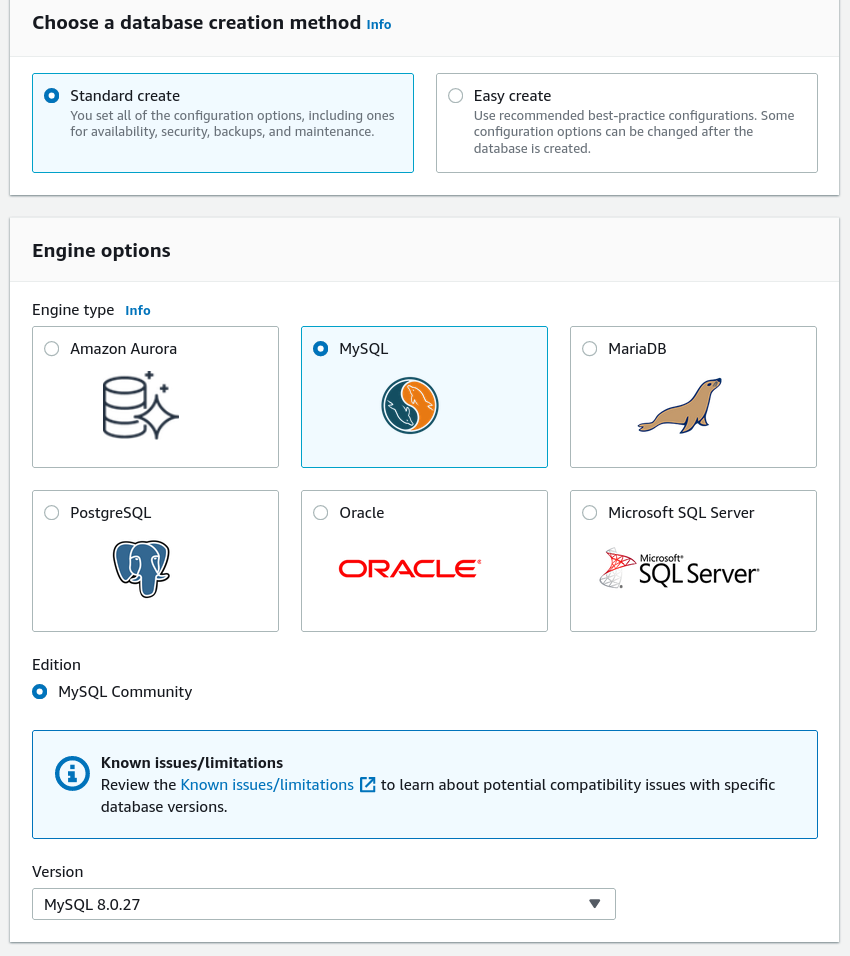
\includegraphics[width=\textwidth]{images/db1}
\end{figure}

For today we are going to use ``Free Tier'' but in the future,
you may wish to explore the different deployment options.
Please peruse the available different options.

\teacher{
  Walk through what Multi-AZ means aka Multiple Availability Zones.
}

\begin{figure}[H]
  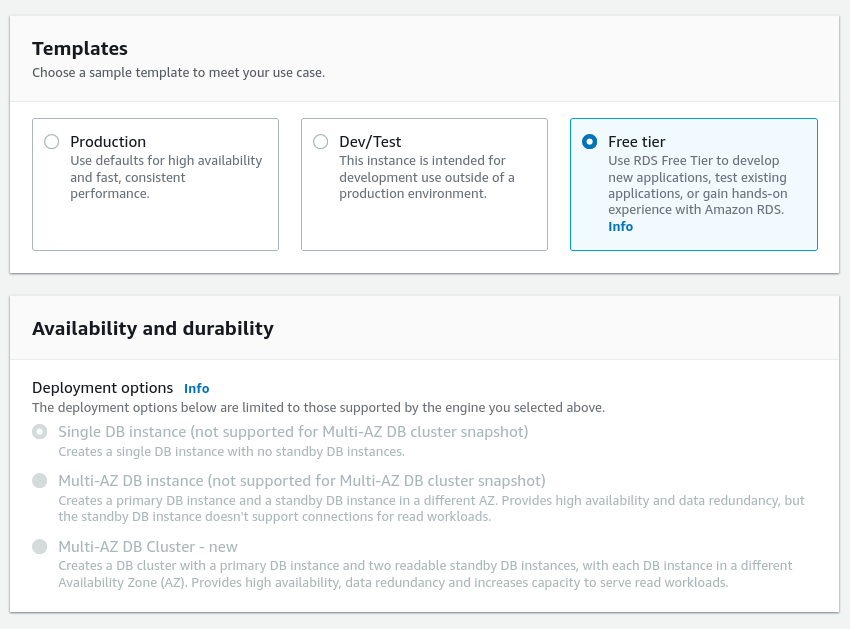
\includegraphics[width=\textwidth]{images/db2}
\end{figure}

Now we need to name our database and create credentials to connect via. Here is where you can enter in credentials for the main account of the database.

\begin{figure}[H]
  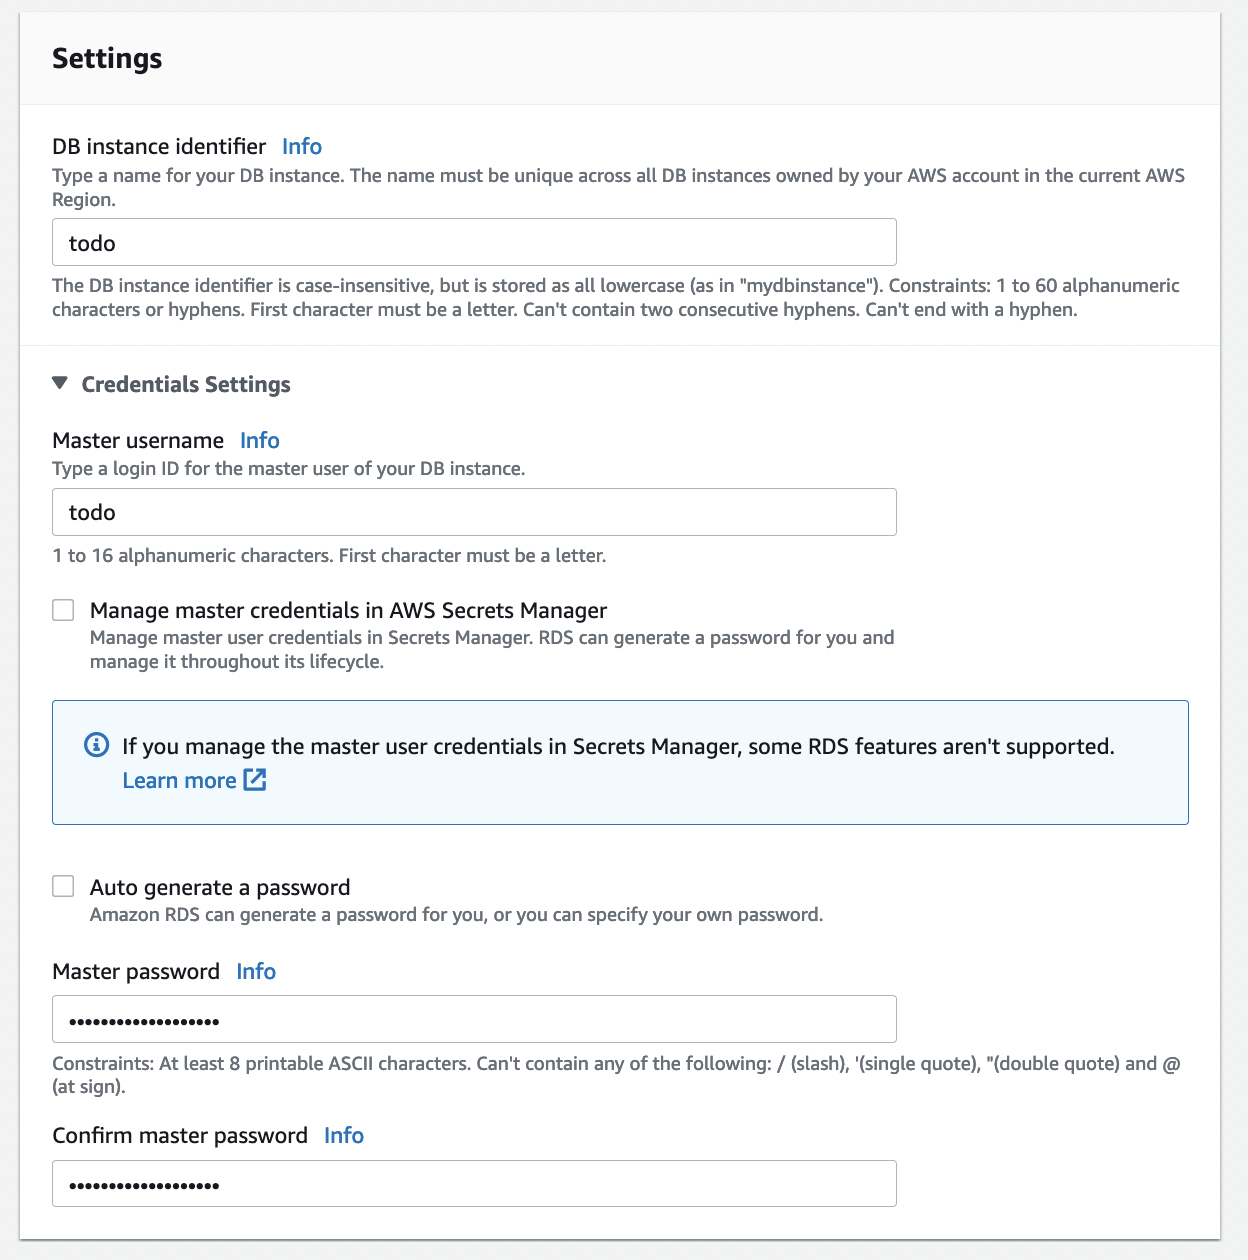
\includegraphics[width=\textwidth]{images/db3}
\end{figure}

For exploring the process select t2.micro, which should be adequate for our needs.

\teacher{
  May want to mention that burstable is not recommended for consistantly used databases.
  Usually DBs are memory focused and thus the standard or memory optimised are used.
}

\begin{figure}[H]
  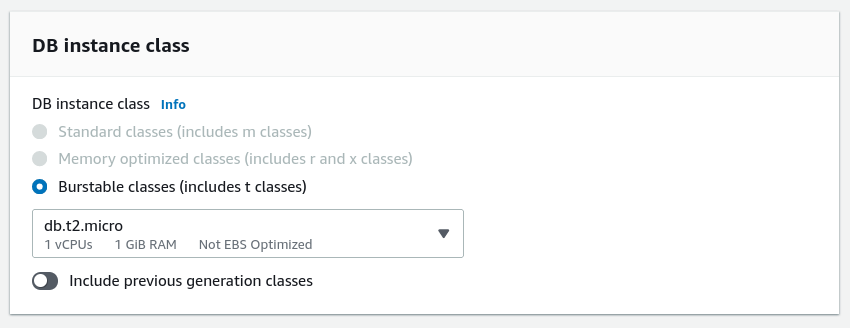
\includegraphics[width=\textwidth]{images/db4}
\end{figure}

For storage we will leave all the default options.

\begin{figure}[H]
  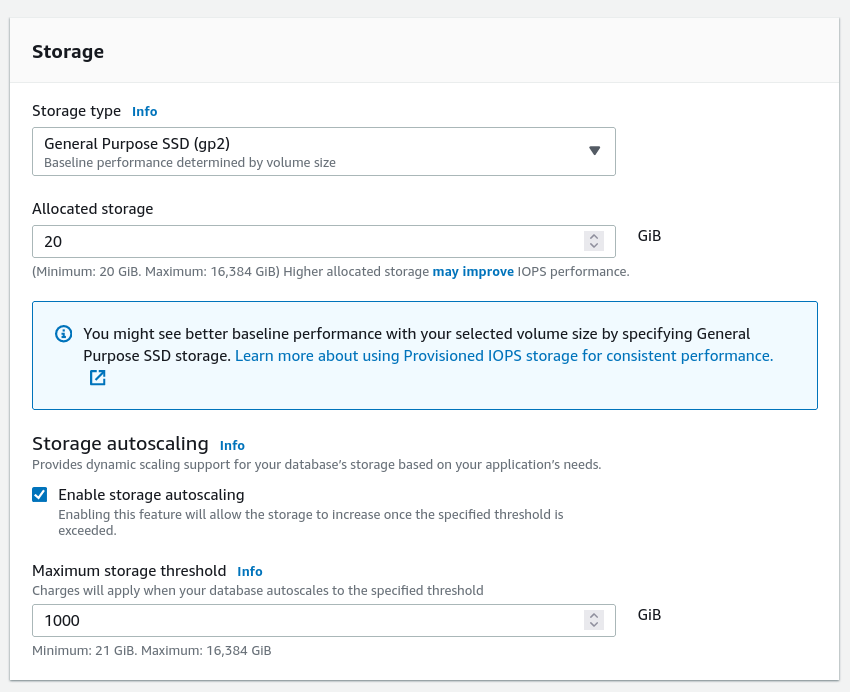
\includegraphics[width=\textwidth]{images/db5}
\end{figure}

In connectivity we need to make sure our instance is publicly available. Usually you do not want to expose your databases publicly and, would instead, have a web server sitting in-front. For our learning purposes though we are going to expose it directly just like we did with our EC2 instances early in the course.

When selecting public access as yes we have to create a new Security Group,
give this Security Group a sensible name.

\begin{figure}[H]
  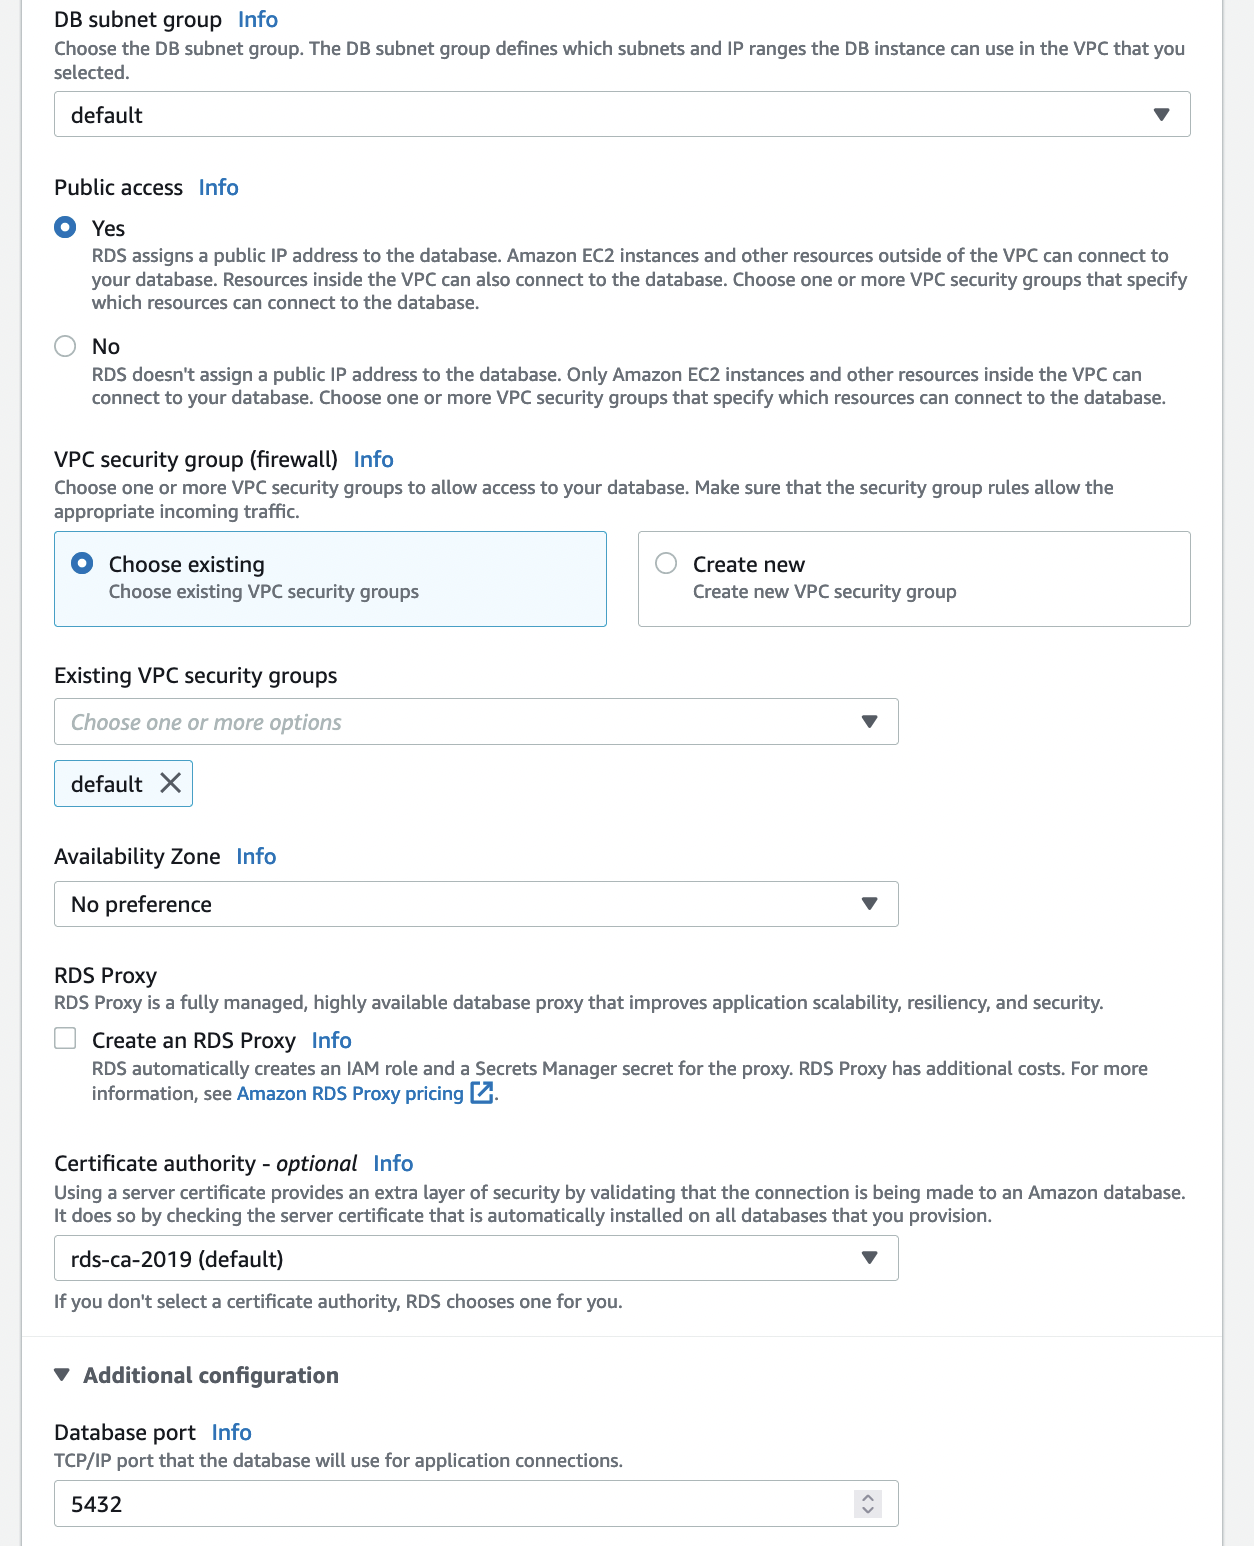
\includegraphics[width=\textwidth]{images/db6}
\end{figure}

We will leave the authentication as password based but we need to expand the ``Additional configuration''. Fill in the ``Initial Database Name'' section to be ``todo'', this is similar to what we had in the Docker Compose's environment variable.

\teacher{
The other options here are to do with the parameters used to start the database,
it is uncommon to have to change these but this is where any settings you would pass in via cli to the db would be set.
}

\begin{figure}[H]
  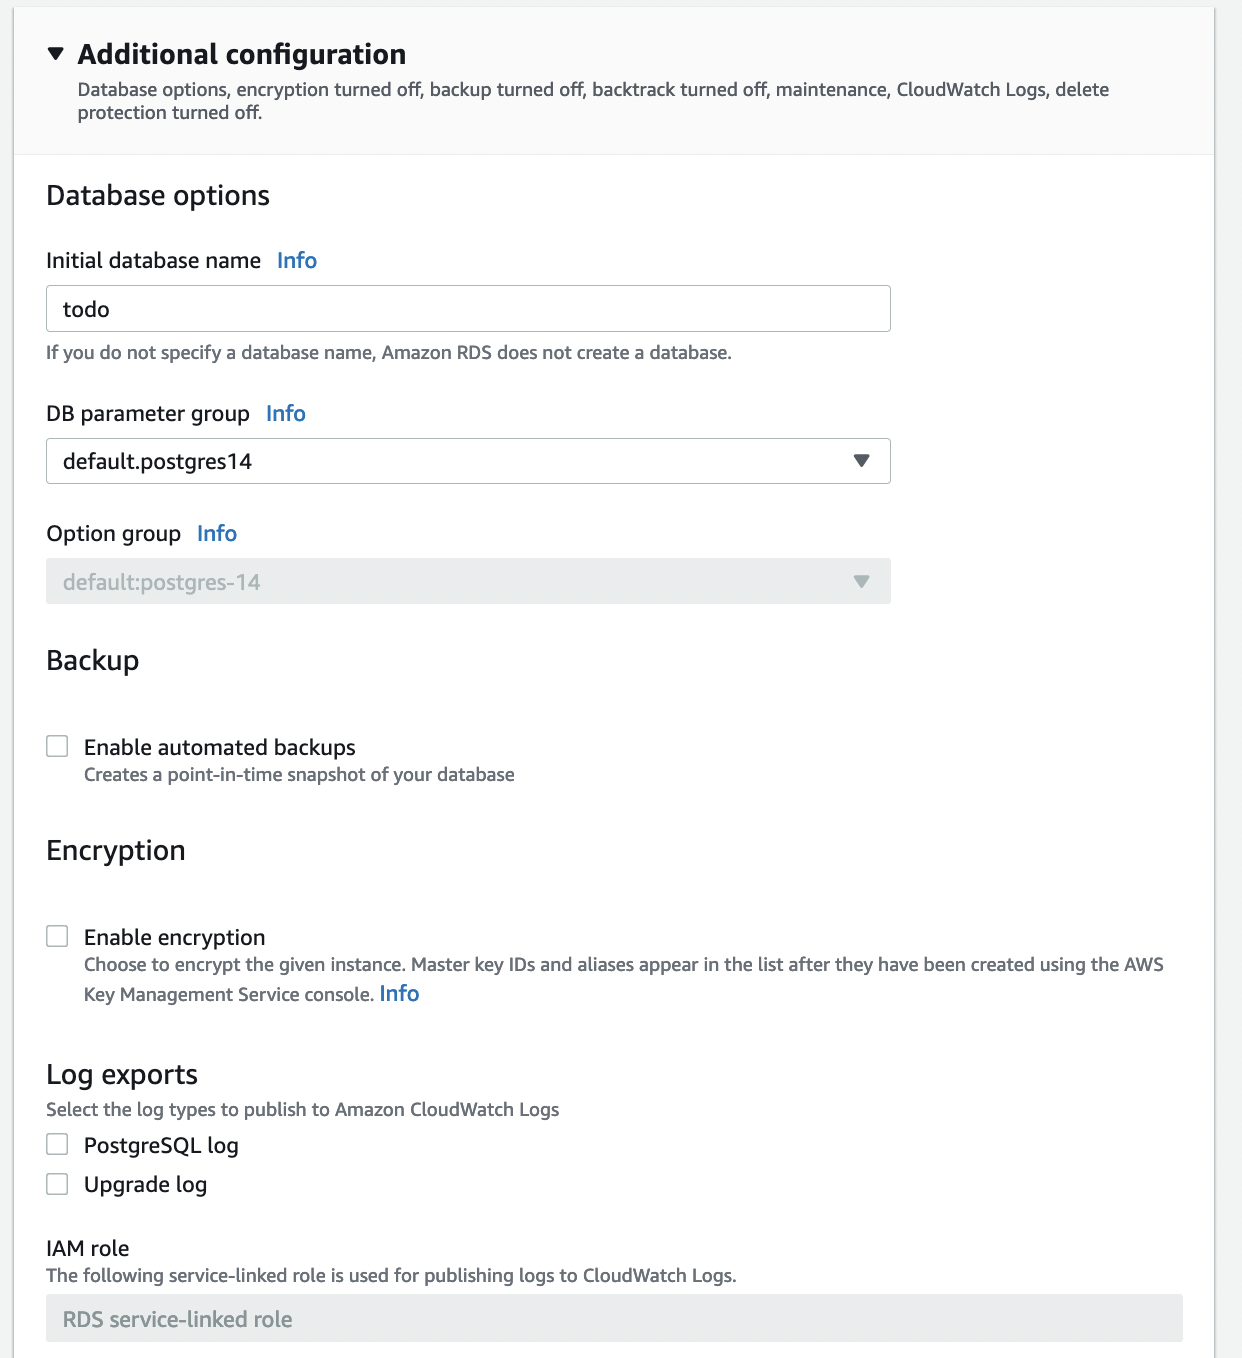
\includegraphics[width=\textwidth]{images/db7}
\end{figure}

Now we can click create which will take some time.

\begin{figure}[H]
  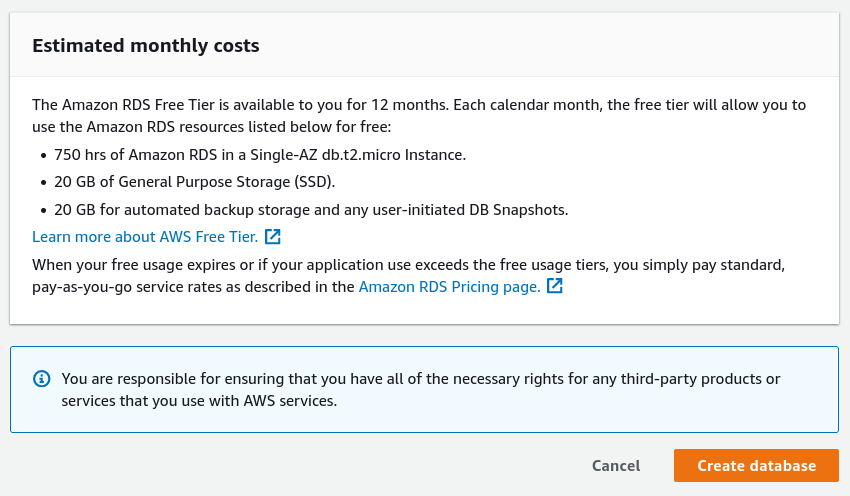
\includegraphics[width=\textwidth]{images/db8}
\end{figure}

Depending on your database it may take 10 to 30 minutes to create, the larger and more complicated the set-up, the longer it usually takes. The database will also do a initial backup when it is created.

\begin{figure}[H]
  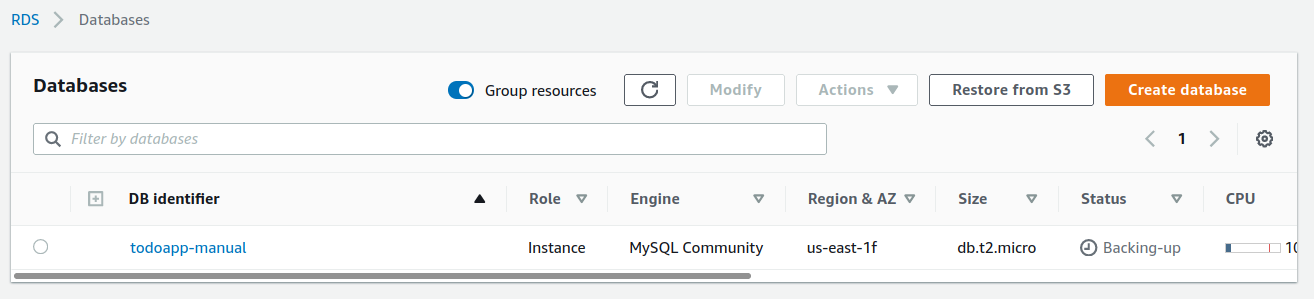
\includegraphics[width=\textwidth]{images/aws_4}
\end{figure}

When the database has finished being created you can select it to view the configuration and details. In this menu we also see the endpoint address which we will need to copy into our Docker Compose file.

\begin{figure}[H]
  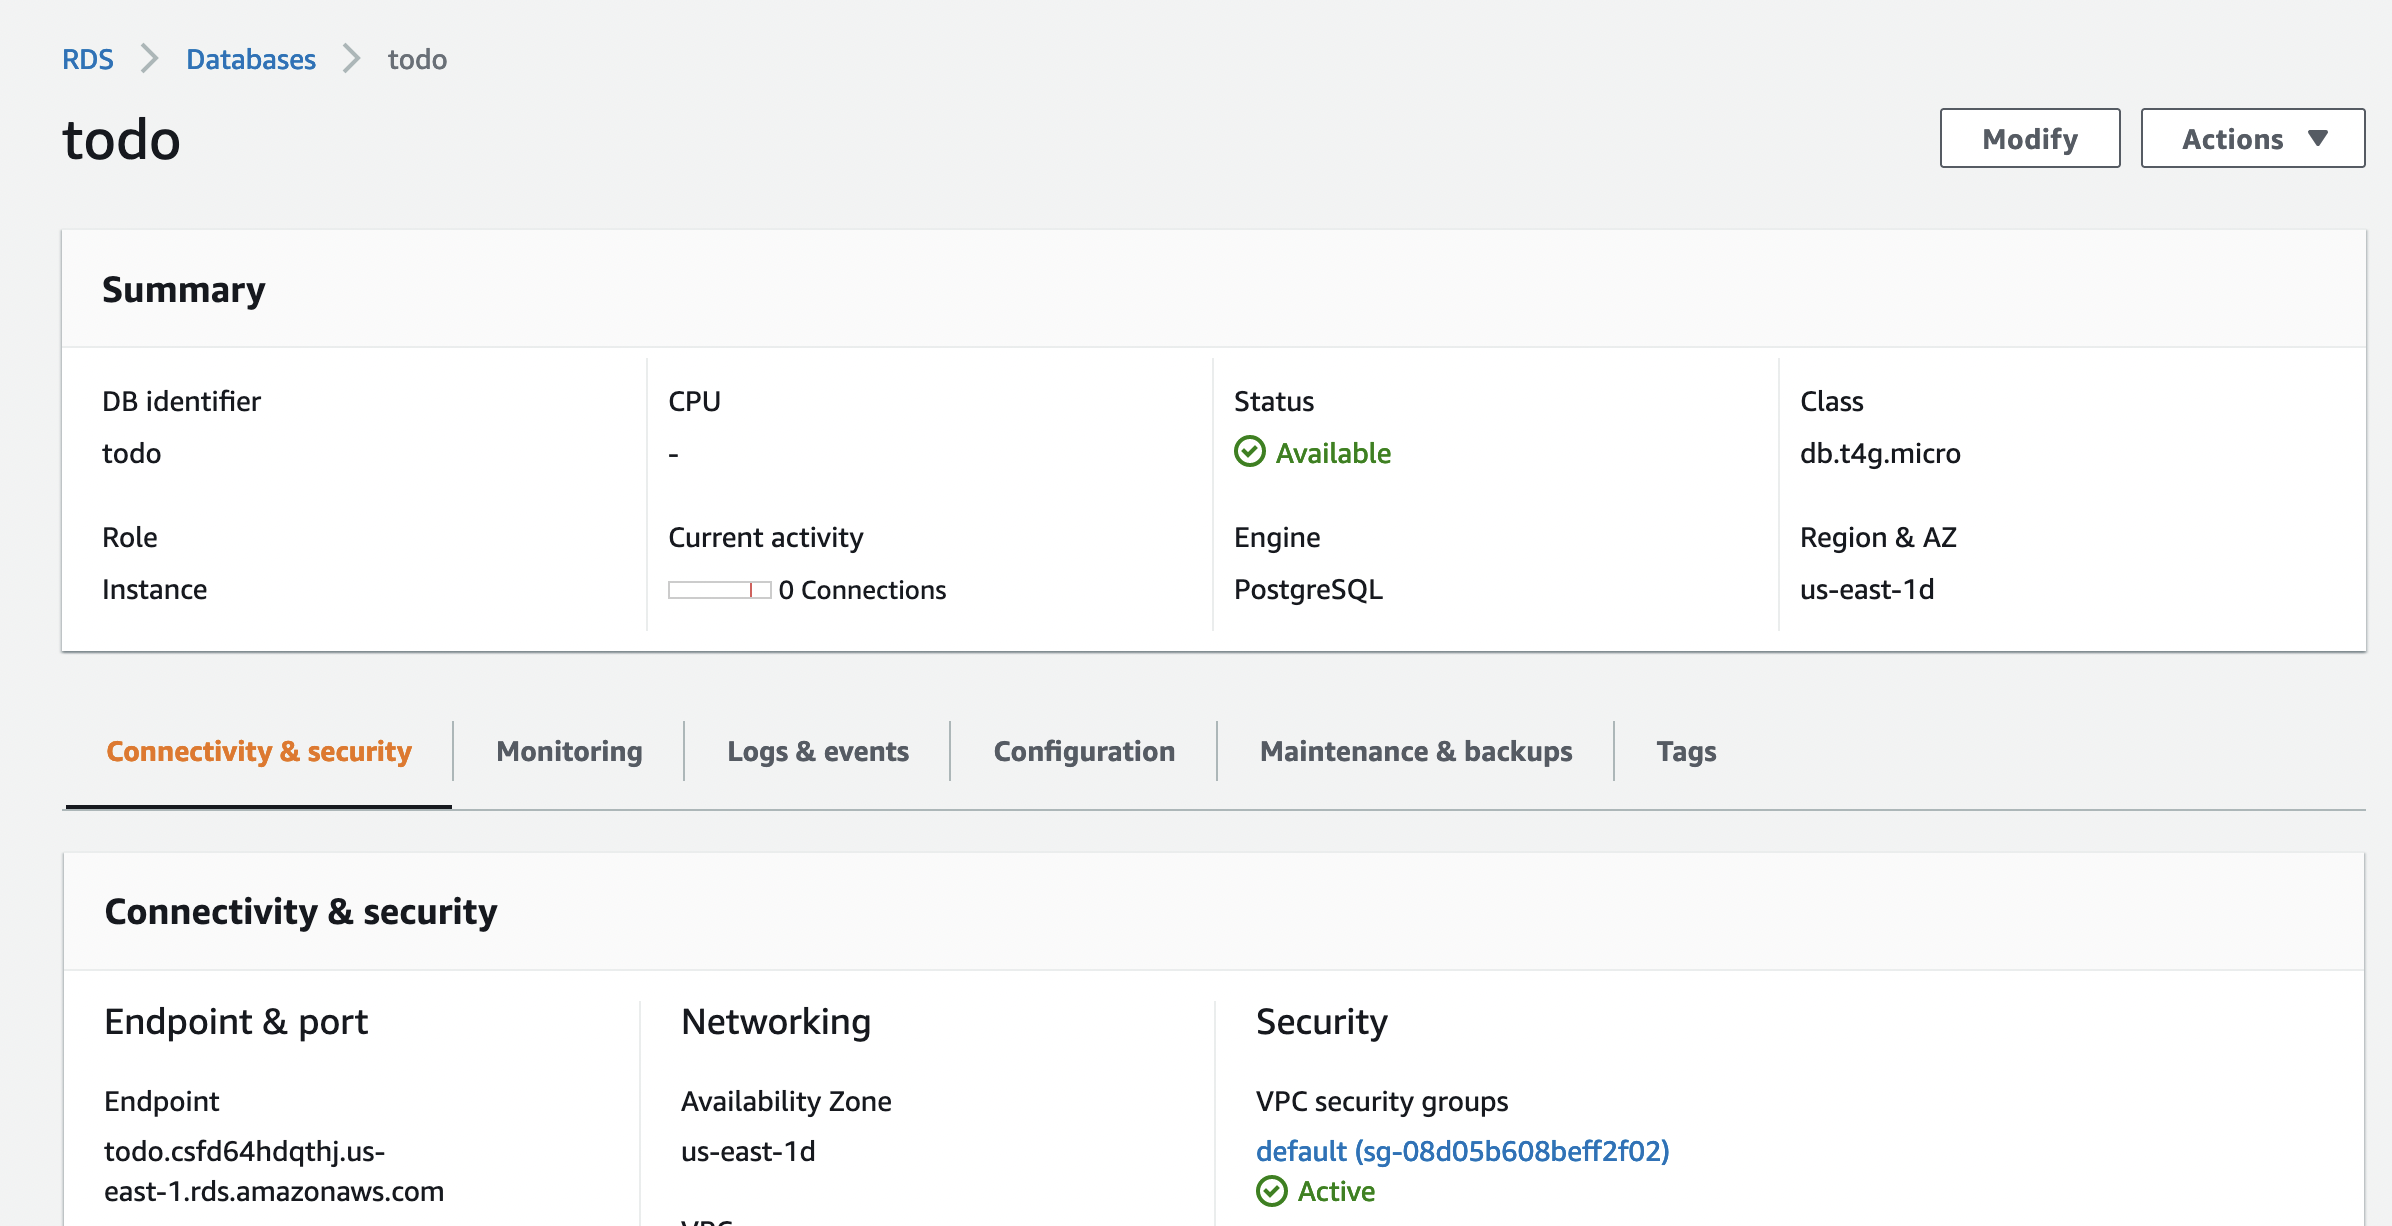
\includegraphics[width=\textwidth]{images/aws_5}
\end{figure}

\section{RDS Database with Terraform}

Now would be a good time to browse the documentation for the RDS database in Terraform:
\url{https://registry.terraform.io/providers/hashicorp/aws/latest/docs/resources/db_instance}.
Using our manual configuration, we can come up with a resource with the appropriate parameters as below:

\begin{code}[language=terraform,numbers=none]{main.tf}
locals {
  password = "foobarbaz" # this is bad
}

resource "aws_db_instance" "todoapp-database" {
  allocated_storage      = 20
  max_allocated_storage  = 1000
  engine                 = "postgres"
  engine_version         = "14"
  instance_class         = "db.t4g.micro"
  db_name                = "todo"
  username               = "todo"
  password               = local.password
  parameter_group_name   = "default.postgres14"
  skip_final_snapshot    = true
  vpc_security_group_ids = [aws_security_group.todo-database.id]
  publicly_accessible    = true

  tags = {
    Name = "todo-database"
  }
}
\end{code}

\noindent Remember to create an appropriate security group as we did through the user interface.

\begin{code}[language=terraform,numbers=none]{main.tf}
resource "aws_security_group" "todo-database" {
  name        = "database"
  description = "Allow inbound Postgresql traffic"

  ingress {
    from_port        = 5432
    to_port          = 5432
    protocol         = "tcp"
    cidr_blocks      = ["0.0.0.0/0"]
  }

  egress {
    from_port        = 0
    to_port          = 0
    protocol         = "-1"
    cidr_blocks      = ["0.0.0.0/0"]
    ipv6_cidr_blocks = ["::/0"]
  }

  tags = {
    Name = "todo-database"
  }
}
\end{code}

\todo{Connect to the database and explore around.}

\section{Container on AWS}

As we mentioned in the Infrastructure as Code notes \cite{iac-notes},
in this course we will use Docker to configure machines and Terraform to configure infrastructure.
AWS has the ability to deploy Docker containers using a service known as Elastic Container Service (ECS). We will cover ECS and deploying maunally via EC2 so you can use the method you feel most confortable with.

For this practical we have made available a Docker container running the todo application which you can use to deploy to AWS. This container is available on Github under the CSSE6400 organisation \url{https://ghcr.io/csse6400/taskoverflow:latest}. This container is very similar to what you have been building in the practicals but contains a simple UI and some extra features for the future practicals.

\subsection{Setup}

Of all the different ways that we can deploy our application we have already decided that we are going to offload the database to AWS. This means that we can move all the "state" of our application away from our containerised environment.

To start off we are going to use what we had above to create a database and the default Terraform. Edit your files so that they match what is provided below:

\begin{code}[language=terraform,numbers=none]{main.tf}
  terraform {
    required_providers {
        aws = {
            source  = "hashicorp/aws"
            version = "~> 4.0"
        }
    }
}

provider "aws" {
    region = "us-east-1"
    shared_credentials_files = ["./credentials"]
    default_tags {
        tags = {
            Course       = "CSSE6400"
            Name         = "TaskOverflow"
            Automation   = "Terraform"
        }
    }
}

locals {
    image             = "ghcr.io/csse6400/taskoverflow:latest"
    database_username = "administrator"
    database_password = "VerySecurePasswordByYourBoiEvan"
}

resource "aws_db_instance" "database" {
  allocated_storage      = 20
  max_allocated_storage  = 1000
  engine                 = "postgres"
  engine_version         = "14"
  instance_class         = "db.t4g.micro"
  db_name                = "todo"
  username               = local.database_username
  password               = local.database_password
  parameter_group_name   = "default.postgres14"
  skip_final_snapshot    = true
  vpc_security_group_ids = [aws_security_group.database.id]
  publicly_accessible    = true
}

resource "aws_security_group" "database" {
  name        = "todo-database"
  description = "Allow inbound Postgres traffic"

  ingress {
    from_port        = 5432
    to_port          = 5432
    protocol         = "tcp"
    cidr_blocks      = ["0.0.0.0/0"]
  }

  egress {
    from_port        = 0
    to_port          = 0
    protocol         = "-1"
    cidr_blocks      = ["0.0.0.0/0"]
    ipv6_cidr_blocks = ["::/0"]
  }
}
\end{code}

The above sets up a RDS instance of Postgres and a security group to allow access to it. We have also added a local variable to store the password for the database. Local variables in Terraform can come through two ways, they can be in a variables block which can be overridden or they can be in a locals block which can be used to store values that are used in multiple places.

Now we can run \texttt{terraform init} and \texttt{terraform apply} to create our database. Once this is done we can move on to the next step. For the next step you must choose a path to follow, either EC2 or ECS, only choose one path for the practical, if you have trouble with one path you can always switch to the other. When switching you should destroy the resources you have created so far before starting the new path.

We recommend that you start with the ECS path as it is the more modern way of deploying containers and is the path that we will be suggesting for the future but all tasks are also doable using EC2.

\subsection{[Path A] EC2}

\aside{
  This is not the recommended path but is provided for those who would like to use EC2 instead of ECS. This is also the path that was used in the first run of the course (2022).
}

\begin{figure}[H]
  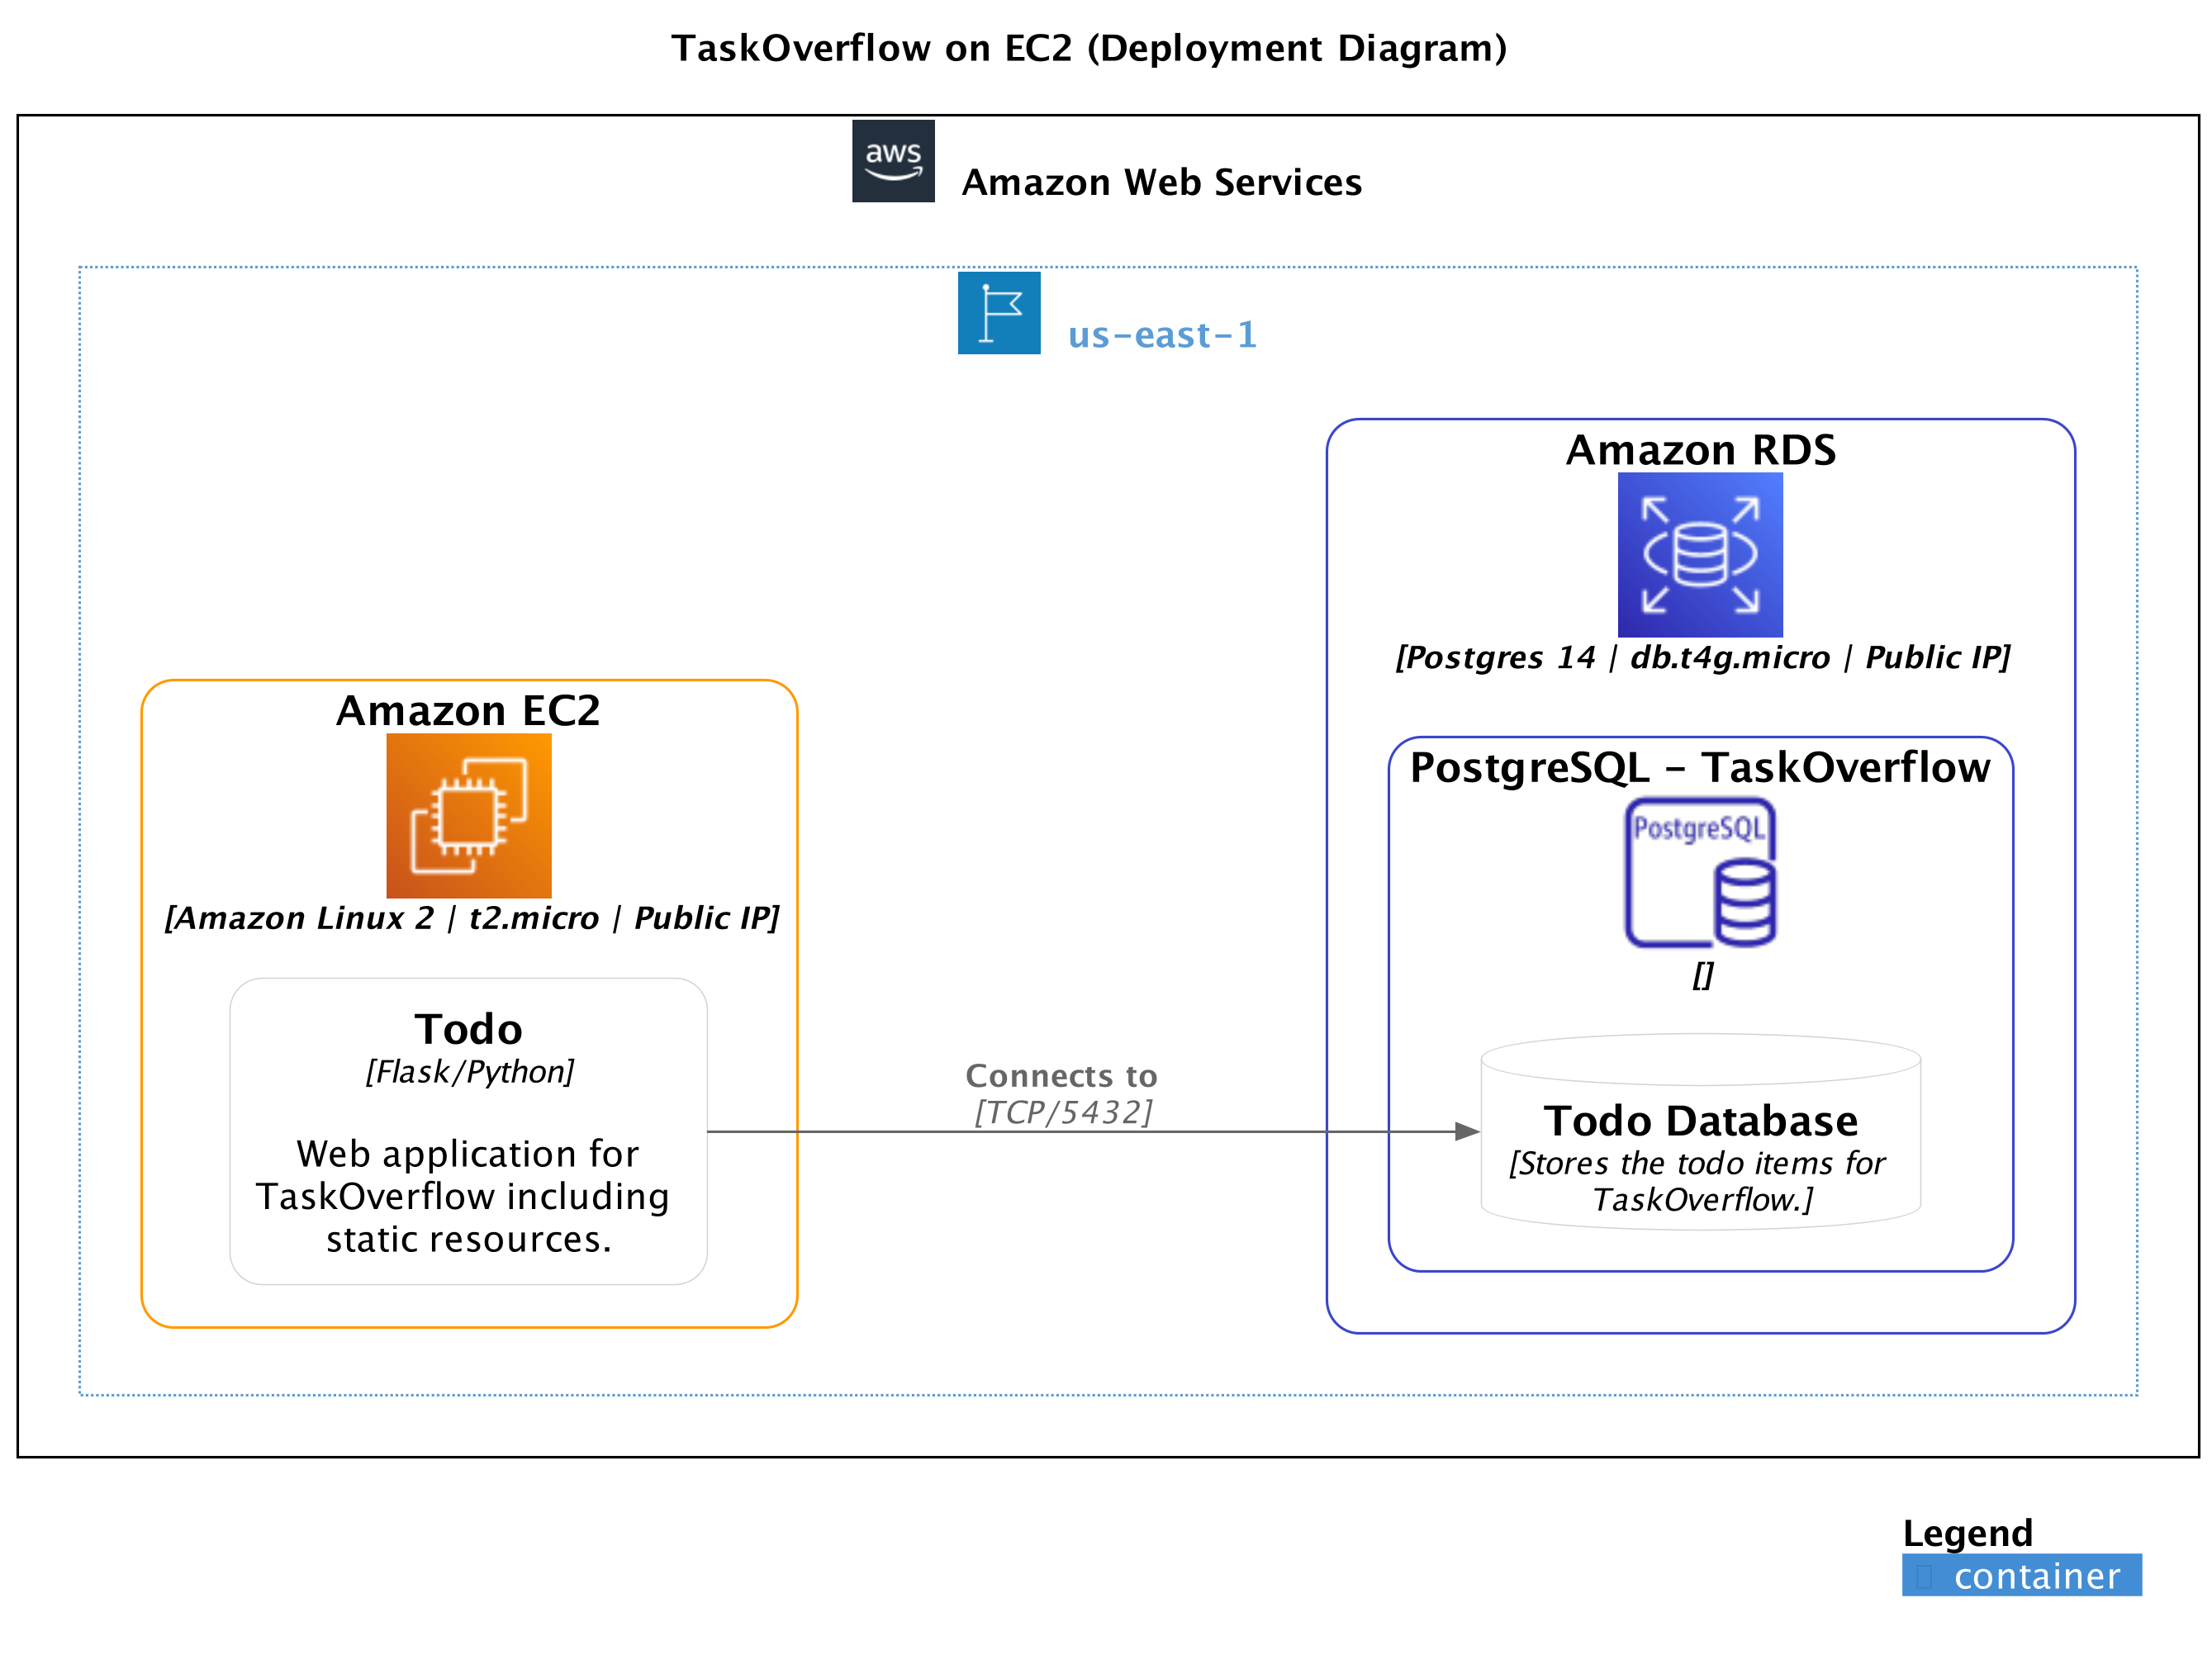
\includegraphics[width=\textwidth]{diagrams/ec2deployment}
\end{figure}

Congrats you have chosen to go down the EC2 path which builds on what we experienced in the previous practicals. To deploy our application we first need to get the EC2 instance running and install Docker on the instance. We can do this by using the following Terraform code:

\begin{code}[language=terraform,numbers=none]{main.tf}
  resource "aws_instance" "todo" {
    ami           = "ami-005f9685cb30f234b" // Amazon Linux 2
    instance_type = "t2.micro"
    key_name      = "vockey" // allows us to SSH into the instance using the preconfigured key
    
    user_data_replace_on_change = true // If we change user_data this will force the box to be recreated
    user_data                   = <<-EOT
  #!/bin/bash
  yum update -y
    EOT
  
    security_groups = [aws_security_group.todo.name] // Firewall for the instance
  }
\end{code}

Compared to the last time we used EC2 instances we have moved the \texttt{user\_data} from a file to being defined in-line and we have made sure to provide the \texttt{key\_name} in case we want to ssh into the deployed instance.

If we ran \texttt{terraform apply} now, our instance would not do anything interesting and we have not defined our security group yet. For the \texttt{user\_data} we need to install Docker and run the container that we have already built. We can do this by changing our \texttt{user\_data}:

\begin{code}[language=terraform,numbers=none]{main.tf}
  user_data                   = <<-EOT
  #!/bin/bash
  yum update -y
  yum install -y docker
  service docker start
  systemctl enable docker
  usermod -a -G docker ec2-user 
  docker run --restart always -e SQLALCHEMY_DATABASE_URI=postgresql://${local.database_username}:${local.database_password}@${aws_db_instance.database.address}:${aws_db_instance.database.port}/${aws_db_instance.database.db_name} -p 6400:6400 ${local.image}
  EOT
\end{code}

The first lines install Docker and start the Docker service and allow the ec2-user to be able to run Docker commands. The last line is where the magic happens by running the container via the Docker cli. To get a refresher about the Docker cli please see the Containers lecture \cite{container-slides} and the \link{Docker documentation}{https://docs.docker.com/}. 

\aside{
  The \texttt{--restart always} flag tells docker to restart the container if it crashes or is stopped. This is useful for our application as it may take a while for the database to be provisioned and we do not want to have to manually restart the container once the database is ready.
}

Now that our instance is ready to go we just need to make sure that it is accessible from the internet. We can do this by creating a security group that allows traffic on port 6400 and attaching it to our instance.

\begin{code}[language=terraform,numbers=none]{main.tf}
  resource "aws_security_group" "todo" {
    name = "todo"
    description = "TaskOverflow Security Group"
  
    ingress {
      from_port = 6400
      to_port = 6400
      protocol = "tcp"
      cidr_blocks = ["0.0.0.0/0"]
    }
  
    ingress {
      from_port = 22
      to_port = 22
      protocol = "tcp"
      cidr_blocks = ["0.0.0.0/0"]
    }
  
    egress {
      from_port = 0
      to_port = 0
      protocol = "-1"
      cidr_blocks = ["0.0.0.0/0"]
    }
  }
\end{code}

Now we can run \texttt{terraform init} and \texttt{terraform apply} to deploy our entire application. Once this is done we can visit the public IP of our instance on port 6400 to see our application running.

\begin{code}[language=terraform,numbers=none]{}
  output "url" {
    value = "http://${aws_instance.todo.public_ip}:6400/"
  }
\end{code}

You should be presented with a very lightweight todo application called TaskOverflow.

\subsubsection{Finished Terraform}

The below is the full terraform we built in this path.

\begin{code}[language=terraform,numbers=none]{main.tf}
  terraform {
    required_providers {
        aws = {
            source  = "hashicorp/aws"
            version = "~> 4.0"
        }
    }
}

provider "aws" {
    region = "us-east-1"
    shared_credentials_files = ["./credentials"]
    default_tags {
        tags = {
            Course       = "CSSE6400"
            Name         = "TaskOverflow"
            Automation   = "Terraform"
        }
    }
}

locals {
    image = "ghcr.io/csse6400/taskoverflow:latest"
    database_username = "administrator"
    database_password = "VerySecurePasswordByYourBoiEvan"
}

resource "aws_db_instance" "database" {
  allocated_storage      = 20
  max_allocated_storage  = 1000
  engine                 = "postgres"
  engine_version         = "14"
  instance_class         = "db.t4g.micro"
  db_name                = "todo"
  username               = local.database_username
  password               = local.database_password
  parameter_group_name   = "default.postgres14"
  skip_final_snapshot    = true
  vpc_security_group_ids = [aws_security_group.database.id]
  publicly_accessible    = true
}

resource "aws_security_group" "database" {
  name        = "todo-database"
  description = "Allow inbound Postgres traffic"

  ingress {
    from_port        = 5432
    to_port          = 5432
    protocol         = "tcp"
    cidr_blocks      = ["0.0.0.0/0"]
  }

  egress {
    from_port        = 0
    to_port          = 0
    protocol         = "-1"
    cidr_blocks      = ["0.0.0.0/0"]
    ipv6_cidr_blocks = ["::/0"]
  }
}

resource "aws_instance" "todo" {
  ami           = "ami-005f9685cb30f234b"
  instance_type = "t2.micro"
  key_name      = "vockey"
  
  user_data_replace_on_change = true
  user_data                   = <<-EOT
#!/bin/bash
yum update -y
yum install -y docker
service docker start
systemctl enable docker
usermod -a -G docker ec2-user 
docker run --restart always -e SQLALCHEMY_DATABASE_URI=postgresql://${local.database_username}:${local.database_password}@${aws_db_instance.database.address}:${aws_db_instance.database.port}/${aws_db_instance.database.db_name} -p 6400:6400 ${local.image}
  EOT

  security_groups = [aws_security_group.todo.name]
}

resource "aws_security_group" "todo" {
  name = "todo"
  description = "TaskOverflow Security Group"

  ingress {
    from_port = 6400
    to_port = 6400
    protocol = "tcp"
    cidr_blocks = ["0.0.0.0/0"]
  }

  ingress {
    from_port = 22
    to_port = 22
    protocol = "tcp"
    cidr_blocks = ["0.0.0.0/0"]
  }

  egress {
    from_port = 0
    to_port = 0
    protocol = "-1"
    cidr_blocks = ["0.0.0.0/0"]
  }
}

output "url" {
  value = "http://${aws_instance.todo.public_ip}:6400/"
}
\end{code}


\subsection{[Path B] ECS}

\aside{
  This is the recommended path for the course and is the path that we will be suggesting for the future.
}

\begin{figure}[H]
  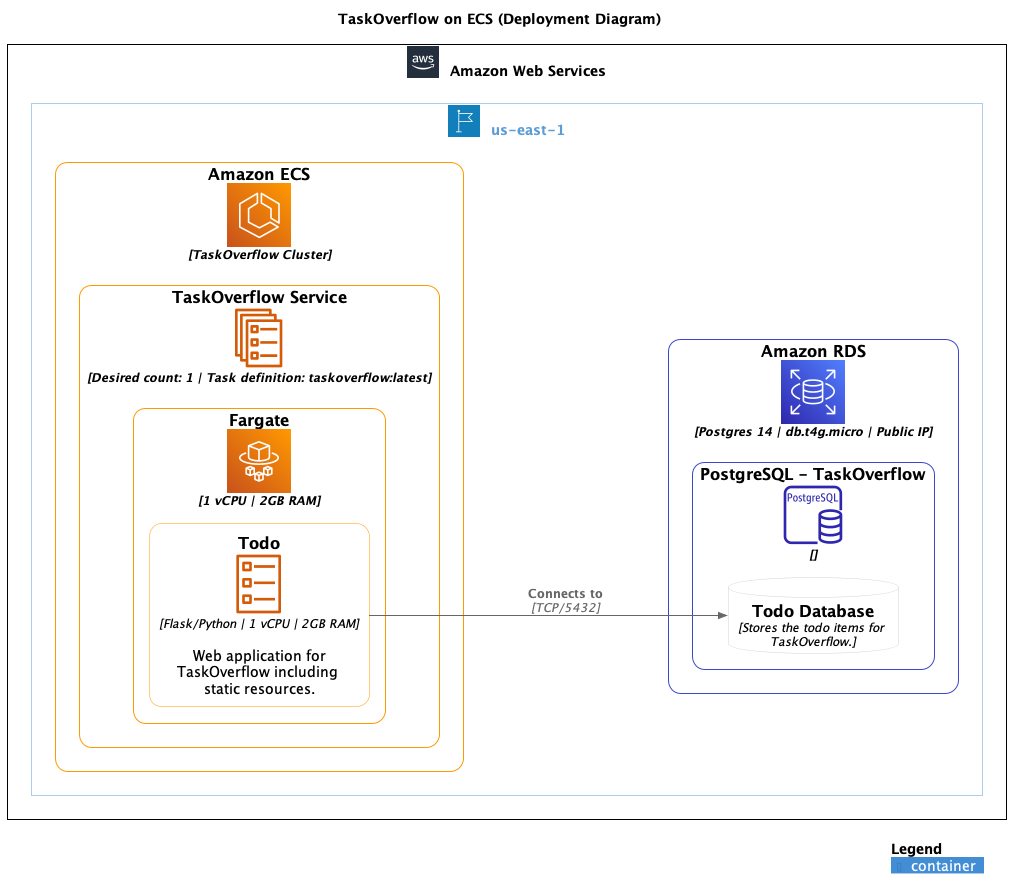
\includegraphics[width=\textwidth]{diagrams/ecsdeployment}
\end{figure}

Congrats you have choosen to go down the ECS path which mimics the same environment that you have via Docker Compose but as a service on AWS. This path is new for the course this year so please let your tutors know of any issues you have.

To start off we need to get some information from our current AWS environment so that we can use it later. Add the below to fetch the IAM role known as LabRole which is a super user in the Lab environments which can do everything you can do through the UI. We will also be fetching the default VPC and the private subnets within that VPC because we need to set-up some networking for our ECS cluster.

\begin{code}[language=terraform,numbers=none,escapechar=!]{}
  data "aws_iam_role" "lab" {
    name = "LabRole"
  }

  data "aws_vpc" "default" {
    default = true
  }

  data "aws_subnets" "private" {
    filter {
      name   = "vpc-id"
      values = [data.aws_vpc.default.id]
    }
  }
\end{code}

The way in Terraform that we can get external information into the environment is by using data sources. These are just like resources but they are not created or destroyed see the below to see the syntactual differences.

\begin{code}[language=terraform,numbers=none,escapechar=!]{}
!\colorbox{yellow}{data}! "aws_iam_role" "lab" {
  ...
}

!\colorbox{yellow}{resource}! "aws_db_instance" "database" {
  ...
}
\end{code}

\begin{code}[language=terraform,numbers=none]{main.tf}
  resource "aws_ecs_task_definition" "todo" {
    family                   = "todo"
    network_mode             = "awsvpc"
    requires_compatibilities = ["FARGATE"]
    cpu                      = 1024
    memory                   = 2048
    execution_role_arn       = data.aws_iam_role.lab.arn
  
    container_definitions = <<DEFINITION
  [
    {
      "image": "${local.image}",
      "cpu": 1024,
      "memory": 2048,
      "name": "todo",
      "networkMode": "awsvpc",
      "portMappings": [
        {
          "containerPort": 6400,
          "hostPort": 6400
        }
      ],
      "environment": [
        {
          "name": "SQLALCHEMY_DATABASE_URI",
          "value": "postgresql://${local.database_username}:${local.database_password}@${aws_db_instance.database.address}:${aws_db_instance.database.port}/${aws_db_instance.database.db_name}"
        }
      ],
      "logConfiguration": {
        "logDriver": "awslogs",
        "options": {
          "awslogs-group": "/taskoverflow/todo",
          "awslogs-region": "us-east-1",
          "awslogs-stream-prefix": "ecs",
          "awslogs-create-group": "true"
        }
      }
    }
  ]
  DEFINITION
  }
\end{code}


\begin{code}[language=terraform,numbers=none]{main.tf}
  resource "aws_ecs_cluster" "taskoverflow" {
    name = "taskoverflow"
  }
\end{code}

\begin{code}[language=terraform,numbers=none]{main.tf}
  resource "aws_ecs_service" "taskoverflow" {
    name            = "taskoverflow"
    cluster         = aws_ecs_cluster.taskoverflow.id
    task_definition = aws_ecs_task_definition.todo.arn
    desired_count   = 1
    launch_type     = "FARGATE"
  
    network_configuration {
      subnets             = data.aws_subnets.private.ids
      security_groups     = [aws_security_group.todo.id]
      assign_public_ip    = true
    }
  }
\end{code}

\begin{code}[language=terraform,numbers=none]{main.tf}
  resource "aws_security_group" "todo" {
    name = "todo"
    description = "TaskOverflow Security Group"
  
    ingress {
      from_port = 6400
      to_port = 6400
      protocol = "tcp"
      cidr_blocks = ["0.0.0.0/0"]
    }
  
    ingress {
      from_port = 22
      to_port = 22
      protocol = "tcp"
      cidr_blocks = ["0.0.0.0/0"]
    }
  
    egress {
      from_port = 0
      to_port = 0
      protocol = "-1"
      cidr_blocks = ["0.0.0.0/0"]
    }
  }
\end{code}

\subsubsection{Finished Terraform}

\begin{code}[language=terraform,numbers=none]{main.tf}
  terraform {
    required_providers {
        aws = {
            source  = "hashicorp/aws"
            version = "~> 4.0"
        }
    }
}

provider "aws" {
    region = "us-east-1"
    shared_credentials_files = ["./credentials"]
    default_tags {
        tags = {
            Course       = "CSSE6400"
            Name         = "TaskOverflow"
            Automation   = "Terraform"
        }
    }
}

locals {
    image = "ghcr.io/csse6400/taskoverflow:latest"
    database_username = "administrator"
    database_password = "VerySecurePasswordByYourBoiEvan"
}

resource "aws_db_instance" "database" {
  allocated_storage      = 20
  max_allocated_storage  = 1000
  engine                 = "postgres"
  engine_version         = "14"
  instance_class         = "db.t4g.micro"
  db_name                = "todo"
  username               = local.database_username
  password               = local.database_password
  parameter_group_name   = "default.postgres14"
  skip_final_snapshot    = true
  vpc_security_group_ids = [aws_security_group.database.id]
  publicly_accessible    = true
}

resource "aws_security_group" "database" {
  name        = "todo-database"
  description = "Allow inbound Postgres traffic"

  ingress {
    from_port        = 5432
    to_port          = 5432
    protocol         = "tcp"
    cidr_blocks      = ["0.0.0.0/0"]
  }

  egress {
    from_port        = 0
    to_port          = 0
    protocol         = "-1"
    cidr_blocks      = ["0.0.0.0/0"]
    ipv6_cidr_blocks = ["::/0"]
  }
}

data "aws_iam_role" "lab" {
  name = "LabRole"
}

resource "aws_ecs_cluster" "taskoverflow" {
  name = "taskoverflow"
}

resource "aws_ecs_task_definition" "todo" {
  family                   = "todo"
  network_mode             = "awsvpc"
  requires_compatibilities = ["FARGATE"]
  cpu                      = 1024
  memory                   = 2048
  execution_role_arn       = data.aws_iam_role.lab.arn

  container_definitions = <<DEFINITION
[
  {
    "image": "${local.image}",
    "cpu": 1024,
    "memory": 2048,
    "name": "todo",
    "networkMode": "awsvpc",
    "portMappings": [
      {
        "containerPort": 6400,
        "hostPort": 6400
      }
    ],
    "environment": [
      {
        "name": "SQLALCHEMY_DATABASE_URI",
        "value": "postgresql://${local.database_username}:${local.database_password}@${aws_db_instance.database.address}:${aws_db_instance.database.port}/${aws_db_instance.database.db_name}"
      }
    ],
    "logConfiguration": {
      "logDriver": "awslogs",
      "options": {
        "awslogs-group": "/taskoverflow/todo",
        "awslogs-region": "us-east-1",
        "awslogs-stream-prefix": "ecs",
        "awslogs-create-group": "true"
      }
    }
  }
]
DEFINITION
}

data "aws_vpc" "default" {
    default = true
}

data "aws_subnets" "private" {
  filter {
    name   = "vpc-id"
    values = [data.aws_vpc.default.id]
  }
}

resource "aws_ecs_service" "taskoverflow" {
  name            = "taskoverflow"
  cluster         = aws_ecs_cluster.taskoverflow.id
  task_definition = aws_ecs_task_definition.todo.arn
  desired_count   = 1
  launch_type     = "FARGATE"

  network_configuration {
    subnets             = data.aws_subnets.private.ids
    security_groups     = [aws_security_group.todo.id]
    assign_public_ip    = true
  }
}

resource "aws_security_group" "todo" {
  name = "todo"
  description = "TaskOverflow Security Group"

  ingress {
    from_port = 6400
    to_port = 6400
    protocol = "tcp"
    cidr_blocks = ["0.0.0.0/0"]
  }

  ingress {
    from_port = 22
    to_port = 22
    protocol = "tcp"
    cidr_blocks = ["0.0.0.0/0"]
  }

  egress {
    from_port = 0
    to_port = 0
    protocol = "-1"
    cidr_blocks = ["0.0.0.0/0"]
  }
}
\end{code}

\subsection{[Path C] EKS / K8S}

This path is not described in the course yet, but we recommend that if you liked the course to have a look at \link{Kubernetes}{https://kubernetes.io/} as it is widely used in industry.

\bibliographystyle{ieeetr}
\bibliography{books,ours}

\end{document}